\documentclass[tikz]{standalone}
\usepackage{pgfplots}
\usepgfplotslibrary{groupplots}
\pgfplotsset{width=7.cm, height=7cm, compat=1.18}
\usepackage{tikz}
\usepackage{circledsteps}
\usepackage{gensymb}
\usepackage{amsmath}
\usepackage[outline]{contour}
\contournumber{64}% default is 16, star form uses 32
\contourlength{.12em}% default is 0.03em
\usetikzlibrary {arrows.meta} 
\usetikzlibrary{decorations.pathreplacing, calligraphy}

\def\myline{very thick}

\begin{document}


\begin{tikzpicture}

\node[anchor=south east, inner sep=0cm] (image) at (canvas cs:x=-1.8cm,y=-0.8cm) {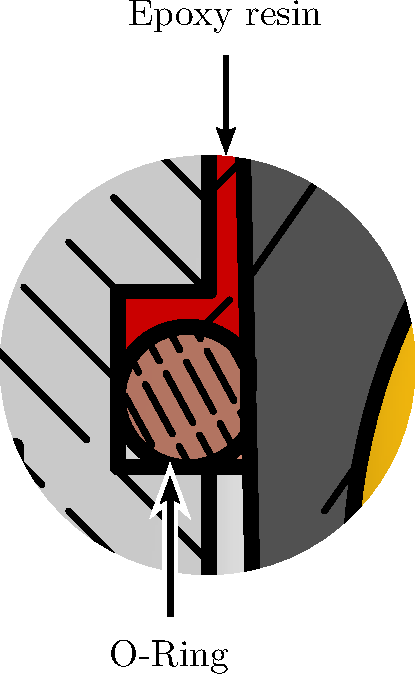
\includegraphics[height=6cm]{test_inset.pdf}};

\begin{groupplot}[group style={group size=2 by 1, horizontal sep=1.5cm}]
%
\nextgroupplot[
legend cell align={left},
legend style={
  fill opacity=1.,
  draw opacity=1,
  text opacity=1,
  at={(0.5,0.30)},
  anchor=center,
  draw=black
},
tick align=outside,
tick pos=left,
xlabel={Time (s)},
xmin=0, xmax=4000,
xtick style={color=black},
ylabel={CO$_2$ (\%)},
ymin=0, ymax=2.7,
ytick style={color=black}
]
\addplot [thick, black]
table {gas_tightness_data/oring.csv};
\addlegendentry{O-Ring}
\addplot [thick, red]
table {gas_tightness_data/epoxy.csv};
\addlegendentry{Epoxy}
\addplot [thick, black, dashed]
table {%
170 0
170 8.1
};
\addlegendentry{CO$_2$ / Air in}
\addplot [thick, black, dashed, forget plot]
table {%
2820 0
2820 8.1
};

\nextgroupplot[
legend cell align={left},
legend style={
	fill opacity=0.8,
	draw opacity=1,
	text opacity=1,
	at={(1.,0.)},
	anchor=south east,
	draw=black,
	xshift=+0.2pt,
	yshift=-0.2pt,
},
tick align=outside,
tick pos=left,
xlabel={Time (s)},
xmin=1000, xmax=2050,
xtick style={color=black},
ymin=0, ymax=2,
ytick style={color=black}
]
\addplot [thick, black]
table {gas_tightness_data/humid_thigh.csv};
\addlegendentry{Human thigh}
\addplot [thick, red]
table {gas_tightness_data/humid_water.csv};
\addlegendentry{Water bath}

\end{groupplot}


\end{tikzpicture}

\end{document}